\documentclass[tikz, border=5mm]{standalone}
\usetikzlibrary{positioning, arrows.meta, calc, patterns, decorations.pathreplacing}

\begin{document}
	
	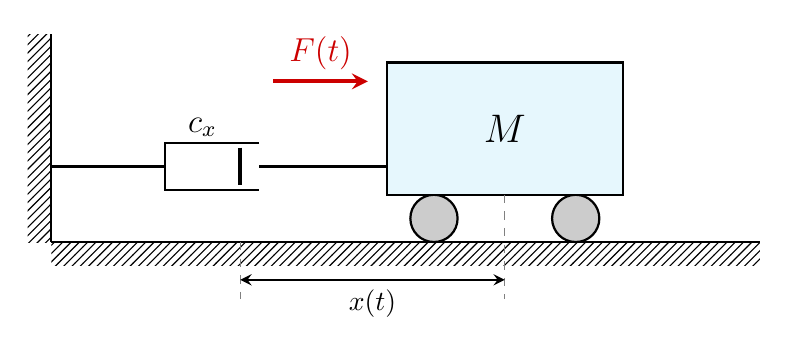
\begin{tikzpicture}[>=stealth, scale=1.2]
		
		% Definición de parámetros geométricos homólogos
		\def\W{2.5}         % Ancho del carro
		\def\H{1.4}         % Alto del carro
		\def\x{3.8}         % Posición x del carro (separado para dar espacio al amortiguador)
		\def\Rrueda{0.25}   % Radio de las ruedas
		\def\Xpared{-1.0}   % Posición horizontal de la pared fija
		
		% --- 1. SUELO Y REFERENCIA FIJA (Estilo idéntico a tu plantilla) ---
		\draw[thick] (\Xpared, 0) -- (6.5, 0);
		\fill[pattern=north east lines] (\Xpared, -0.25) rectangle (6.5, 0);
		
		% Pared rígida de apoyo izquierda
		\draw[thick] (\Xpared, 0) -- (\Xpared, 2.2);
		\fill[pattern=north east lines] (\Xpared-0.25, 0) rectangle (\Xpared, 2.2);
		
		% --- 2. EL AMORTIGUADOR VISCOSO (cx) ---
		\def\Ydamper{0.8}   % Altura central del amortiguador
		
		% Líneas de conexión del amortiguador
		\draw[thick] (\Xpared, \Ydamper) -- (\Xpared+1.2, \Ydamper); % Desde pared al cilindro
		\draw[thick] (\x - \W/2, \Ydamper) -- (\Xpared+2.2, \Ydamper); % Desde el carro al pistón
		
		% Cilindro exterior del amortiguador (Carcasa)
		\draw[thick] (\Xpared+2.2, \Ydamper+0.25) -- (\Xpared+1.2, \Ydamper+0.25) -- (\Xpared+1.2, \Ydamper-0.25) -- (\Xpared+2.2, \Ydamper-0.25);
		
		% Émbolo/Pistón interior móvil
		\draw[line width=1.5pt] (\Xpared+2.0, \Ydamper+0.2) -- (\Xpared+2.0, \Ydamper-0.2);
		
		% Etiqueta del coeficiente de fricción
		\node[above=0.25cm, font=\large] at (\Xpared+1.6, \Ydamper) {$c_x$};
		
		% --- 3. EL CARRO (M) ---
		% Ruedas (Gris fill=gray!40)
		\draw[thick, fill=gray!40] (\x - \W/2 + 0.5, \Rrueda) circle (\Rrueda);
		\draw[thick, fill=gray!40] (\x + \W/2 - 0.5, \Rrueda) circle (\Rrueda);
		
		% Cuerpo del carro (Azul fill=cyan!10)
		\draw[thick, fill=cyan!10] (\x - \W/2, 2*\Rrueda) rectangle (\x + \W/2, 2*\Rrueda + \H);
		\node at (\x, 2*\Rrueda + \H/2) {\Large $M$};
		
		% --- 4. FUERZA APLICADA Y COTAS ---
		% Fuerza neta F(t) (Flecha gruesa idéntica a tu variable u)
		\draw[->, line width=1.5pt, red!80!black] (\x - \W/2 - 1.2, 2*\Rrueda + \H - 0.2) -- ++(1.0, 0) node[midway, above] {\large $F(t)$};
		
		% Cota de posición x con línea discontinua de referencia
		\draw[dashed, gray] (\x, 2*\Rrueda) -- (\x, -0.6);
		\draw[dashed, gray] (1.0, 0) -- (1.0, -0.6); % Origen virtual para la cota
		\draw[<->, thick] (1.0, -0.4) -- (\x, -0.4) node[midway, below] {$x(t)$};
		
	\end{tikzpicture}
	
\end{document}